\documentclass{article}

\usepackage{amsmath}
\usepackage[usenames,dvipsnames]{color}
\usepackage{listings}
\usepackage[a4paper, top=2cm, bottom=3cm, left=2cm, right=2cm]{geometry}
\usepackage{graphicx}

\usepackage{tikz}
\usetikzlibrary{arrows,shapes,shapes.multipart,shapes.geometric,
	snakes,automata,backgrounds,petri,calc,positioning}

\newcommand{\bfc}{{\sc Bfc}}
\newcommand{\mist}{{\sc Mist}}
\newcommand{\iic}{{\sc IIC}}
\newcommand{\pnerf}{{\sc Pnerf}}
\newcommand{\zthree}{{\sc Z3}}
\newcommand{\ttt}[1]{\texttt{#1}}
 
\tikzstyle{place}=[circle,thick,draw=black!75,fill=white!20,
  	minimum size=6mm]
\tikzstyle{red place}=[place,draw=red!75,fill=red!20]
\tikzstyle{blue place}=[place,draw=blue!75,fill=blue!20]
\tikzstyle{transition}=[rectangle,thick,draw=black!75,
  	fill=black!20,minimum size=4mm]

\tikzstyle{state}=[draw, ellipse, aspect=2]
\tikzstyle{action}=[draw, rectangle, align=center]
\tikzstyle{decision}=[draw, diamond, aspect=2, align=center]
\tikzstyle{print}=[draw, trapezium, trapezium left angle=70, trapezium right angle=-70]
\tikzstyle{every edge}=[draw, ->, >=stealth, shorten >=2pt, shorten <=2pt]

\begin{document}

\title{Report on a Safety Checker for Petri nets}
\author{Philipp Meyer \and Rusl\'{a}n Ledesma-Garza}
% \institute{Technische Universit\"at M\"unchen}
\date{Mon Nov 25 14:24:10 CET 2013}



\section{Preliminaries}


\begin{verbatim}
* Petri net:
 N = (S, T, E, M0), where
 S : places
 T : transitions
 E : edges
 M0: initial marking

* Property:
 P, linear arithmetic formula
\end{verbatim}
\iffalse
\begin{verbatim}
 Examples:
  x + y < 0
  x + y < 0 \\and x + z > 0
  x + y < 0 \\or  x + z > 0

 ~P = (x + y <  0 \\and x + z >  0) \\or  x + z >  0
  P = (x + y >= 0 \\or  x + z <= 0) \\and x + z <= 0
\end{verbatim}
\fi

\newpage
\section{Method Safety}

The method Safety checks that a given Petri net \verb=N= never violates a property \verb=P=.
We present the method Safety by example on Lamport's 1-bit algorithm [Esparza1997].

\begin{verbatim}
* Code

TODO

* Property: Thread 1 and Thread 2 are never in the critical section at the same time.

* Petri net:

\end{verbatim}

\begin{center}
  \includegraphics[width=12cm]{lamport}
\end{center}

\begin{verbatim}
* Property P: cs1 + cs2 <= 1
\end{verbatim}

\newpage
\begin{verbatim}
* Method Safety:

  Subprocedure \mathcal{C} constructs state constraints C corresponding to N.
\end{verbatim}

\begin{center}
  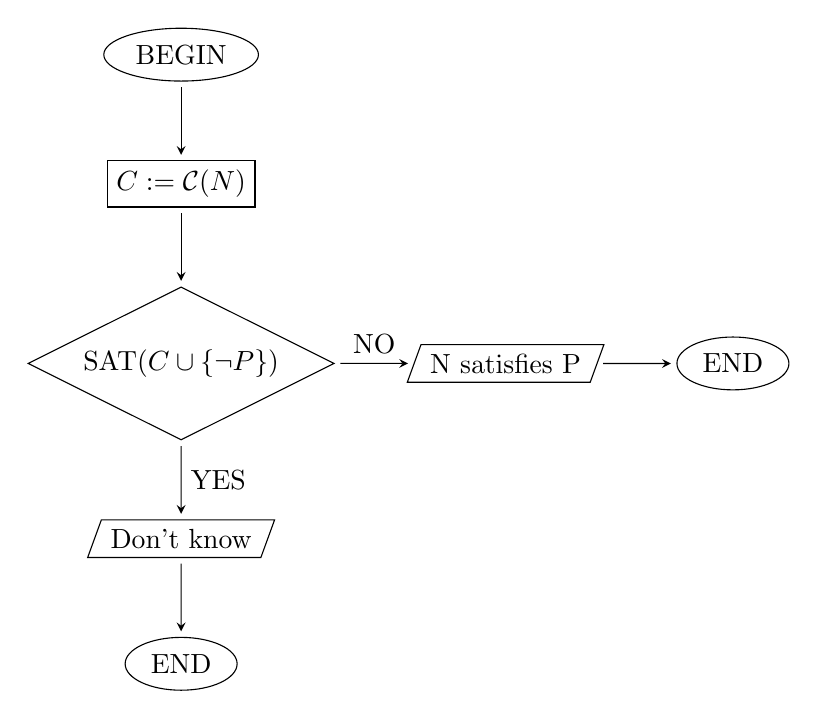
\begin{tikzpicture}
    \node[state] (begin) {BEGIN};
    \node[action, below=of begin] (c) {$C:=\mathcal C(N)$};
    \node[decision, below=of c] (satc) {$\text{SAT}(C \cup \{\neg P\})$};
    \node[print, right=of satc] (yes) {N satisfies P};
    \node[print, below=of satc] (dontknow) {Don't know};
    \node[state, right=of yes] (end1) {END};
    \node[state, below=of dontknow] (end2) {END};
    
    \draw (begin) edge (c);
    \draw (c) edge (satc);
    \draw (satc) edge node[above]{NO} (yes);
    \draw (yes) edge (end1);
    \draw (satc) edge node[right]{YES} (dontknow);
    \draw (dontknow) edge (end2);
  \end{tikzpicture}
\end{center}

\begin{verbatim}
* Property of state constraints C: If C U {\neg P} is unsat then N |= P.

* Example:
  - State constraints C:

    Place equations:
  
    id1        = 1 + u1 - u2
    ^            ^   ^    ^
    |            |   |    |
    |            |   |    |
    |            |   |    |
    |            |   |   # of tokens taken from nc
    |            |   |    
    |            |  # of tokens given to nc
    |            |
    |          initial number of tokens in nc
    |
    number of tokens in nc

    cs1        = 0 - u1      + u3
    idle1      = 1 + u1 - u2
    req1       = 0      + u2 - u3
    nid1       = 0 - u1 + u2
    id2        = 1                     + v2           + v5 - v6
    cs2        = 0                               + v4 - v5
    idle2      = 1                          + v3 + v5      - v6
    req2       = 0                - v1           - v4      + v6
    after_you2 = 0                + v1 - v2
    await2     = 0                     + v2 - v3
\end{verbatim}

\newpage

\begin{verbatim}
    Non-negativity conditions:
  
    id1        >= 0
    cs1        >= 0
    idle1      >= 0
    req1       >= 0
    nid1       >= 0
    id2        >= 0
    cs2        >= 0
    idle2      >= 0
    req2       >= 0
    after_you2 >= 0
    await2     >= 0
    u1         >= 0
    u2         >= 0
    u3         >= 0
    v1         >= 0
    v2         >= 0
    v3         >= 0
    v4         >= 0
    v5         >= 0
    v6         >= 0

  - Negated Property \neg P:

    cs1 + cs2  >= 2

* Place equation:
  
  For a given place s the place equation is

  # of tokens in s = initial number of tokens of place s
                     + # times each input transition of s fires
                     - # times each output transition of s fires

* Non-negativity conditions:

  # of tokens in place s           >= 0
  # of times transition t is fired >= 0

* Subprocedure \mathcal{C}:

  Input:
    (S, T, E, M0) : Petri net
  Output:
    C : State constraints
  Pseudocode:
  
  # Place equations
  for s in S:
    # initial number of tokens
    print(s + " = " + M0(s)"
    for t in T:
      if (t, s) in E and not (s, t) in E:
        # input transition
        print(" + " + t)
      if (s, t) in E and not (t, s) in E:
        # output transition
        print(" - " + t)
    print("\n")
  
  # Non-negativity conditions
  for s in S:
    print(s + " >= 0\n")
  for t in T:
    print(t + " >= 0\n")
\end{verbatim}

\iffalse

\newpage
\section{Method Invariant}

The method Invariant constructs an invariant \verb=I= for given Petri net \verb=N= and \verb=P= when \verb=N= never violates \verb=P=.
We present the method Invariant by example on a simplified mutual exclusion algorithm by Delzanno2001.

\begin{verbatim}
* Code, property, and Petri net: same as in section Method Safety.
\end{verbatim}

\begin{verbatim}
* Method Invariant

  Subprocedure \mathcal{C'} constructs dual state constraints C' corresponding to N and P.
  Subprocedure Model returns assignment A such that A satisfies C'.
  Subprocedure Inv constructs invariant I corresponding to N and A.
\end{verbatim}

\begin{center}
  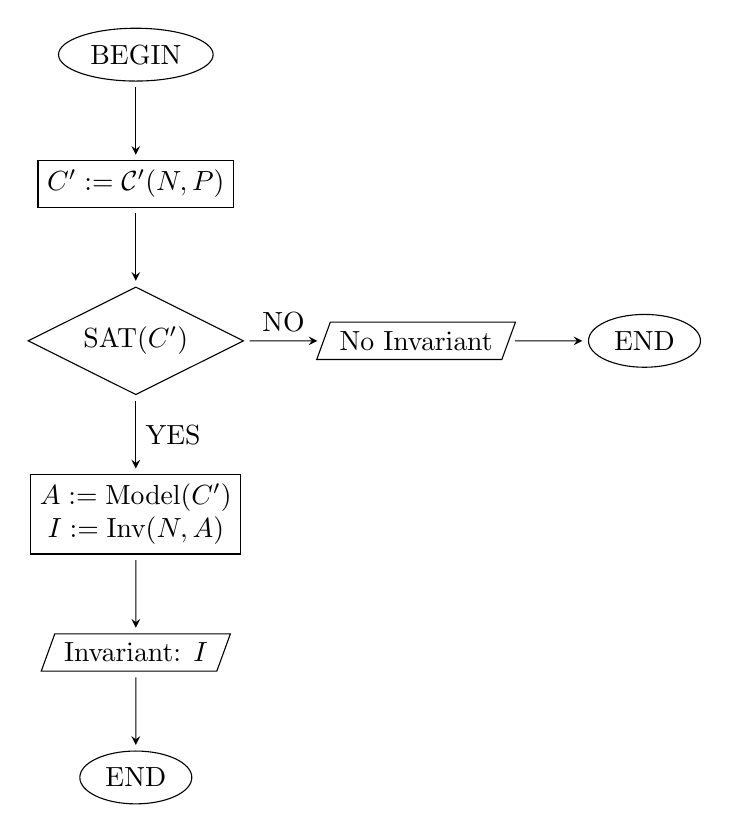
\begin{tikzpicture}
    \node[state] (begin) {BEGIN};
    \node[action, below=of begin] (c) {$C':=\mathcal C'(N, P)$};
    \node[decision, below=of c] (satc) {$\text{SAT}(C')$};
    \node[print, right=of satc] (noinv) {No Invariant};
    \node[action, below=of satc] (inv) {$A:=\text{Model}(C')$\\
      $I := \text{Inv}(N, A)$};
    \node[print, below=of inv] (printinv) {Invariant: $I$};
    \node[state, right=of noinv] (end1) {END};
    \node[state, below=of printinv] (end2) {END};
    
    \draw (begin) edge (c);
    \draw (c) edge (satc);
    \draw (satc) edge node[above]{NO} (noinv);
    \draw (satc) edge node[right]{YES} (inv);
    \draw (noinv) edge (end1);
    \draw (inv) edge (printinv);
    \draw (printinv) edge (end2);
  \end{tikzpicture}
\end{center}

\begin{verbatim}
* Property of dual state constraints C':  If C' is sat then N |= P.

* Property of invariant I:
  - I is reachable: For each reachable marking M, I(M) is valid
  - I is safe:      For markings that violate the property, I(M) is unsat
  - I is inductive: For each marking M, if I(M) is valid and M -> M1 then I(M1) is valid
\end{verbatim}

\newpage
\begin{verbatim}
* Example:
  - Dual state constraints C':

    - nc - m + cs1 <= 0
    - nc - m + cs2 <= 0
      nc + m - cs1 <= 0
      nc + m - cs2 <= 0

    2 \cdot nc + m < 2 \cdot target1

    Non-negativity conditions:

    target1 >= 0
    nc      >= 0
    m       >= 0
    cs1     >= target1
    cs2     >= target1
  
  - Model A:

    target1 = 1
    nc      = 0
    m       = 1
    cs1     = 1
    cs2     = 1
    
  - Invariant:

    cs1 + cs2 + m <= 1

\end{verbatim}

\newpage
\begin{verbatim}
* Derivation of invariant I for Petri net N that satisfies property P:

  M                                    : marking          ~ places
  C                                    : incidence matrix ~ rows correspond to places, columns correspond to transitions, relates places to transitions
  X                                    : firing vector    ~ transitions

  The following constraints C1 are unsat.
  M = M0 + C*X                         : place equations
  M >= 0                               : non-negativity conditions for places
  X >= 0                               : non-negativity conditions for transitions
  AM >= b                              : property P negated

  Substitute M to obtain constraints C2.
  A(M0 + CX) >= b                      : property P negated
  M0 + CX >= 0                         : non-negativity conditions for places
  X >= 0                               : non-negativity conditions for transitions

  Rewrite each system to obtain constraints C3.
  (-A*C)      (A*M0-b)                 : property P negated
  (  -C)*X <= (  M0  )                 : non-negativity conditions for places
  (  -I)      (   0  )                 : non-negativity conditions for transitions

  Apply Farkas' Lemma to obtain constraints C4.
  yT*(-A*C)                            : 
     (  -C) = 0                        : 
     (  -I)                            : 

  yT*(A*M0-b)                          : 
     (  M0  ) < 0                      : 
     (   0  )                          : 

  y >= 0                               : 

  The constraints C4 are sat iff the following constraints C5 are sat.
  y1 * A * C + y2 * C + y3 = 0         : 
  y1 * (A*M - b) + y2 * M0 < 0         : 
  y1 >= 0                              : 
  y2 >= 0                              : 
  y3 >= 0                              : 

  The constraints C5 are sat iff the following constraints C6 are sat.
  (y1 * A + y2) * C  <= 0              : 
  (y1 * A + y2) * M0 < y1 * b          : 
  y1 >= 0                              : 
  y2 >= 0                              : 

  The constraints C6 are sat iff the following constraints C' are sat.
  \lambda * C  <= 0                    : inductivity constraint
  \lambda * M0 < y1 * b                : safety constraint
  \lambda >= y1 * A                    : property constraint
  y1 >= 0                              : non-negativity constraint

  For \lambda satisfying C' the invariant is the following.
  I(M) = (\lambda * M <= \lambda * M0) : invariant
\end{verbatim}

\newpage
\begin{verbatim}
* Subprocedure \mathcal{C'}:

  Input:
    (S, T, E, M0) : Petri net
    P             : Property
  Output:
    C'            : Dual state constraints

Input:
 N = (S, T, E, M0)
   = ( (nc m cs1 cs2) (t1 t2 t3 t4) (e1 ... en) (2 1 0 0) )
 P = ( cs1 + cs2 <= 1 )

TODO: Unroll pseudocode?


* Subprocedure Inv:

  Input:
    (S, T, E, M0) : Petri net
    A             : Satisfying assignment for C'

  Output:
    I             : Invariant

TODO: Unroll pseudocode?
\end{verbatim}

\newpage
\section{Method Invariant with Minimization}

The method Invariant with Minimization constructs an invariant \verb=I=
that uses a minimal number of places for given Petri net \verb=N= and
\verb=P= when \verb=N= never violates \verb=P=. 
We present the method Invariant with Minimization by example on a
simplified mutual exclusion algorithm by Delzanno2001.

\begin{verbatim}
* Code, property, and Petri net: same as in section Method Safety.
\end{verbatim}

\begin{verbatim}
* Method Invariant with Minimization

  Subprocedure \text{MinConstraints} constructs minimization constraints C_M corresponding to N and A
\end{verbatim}

\begin{center}
  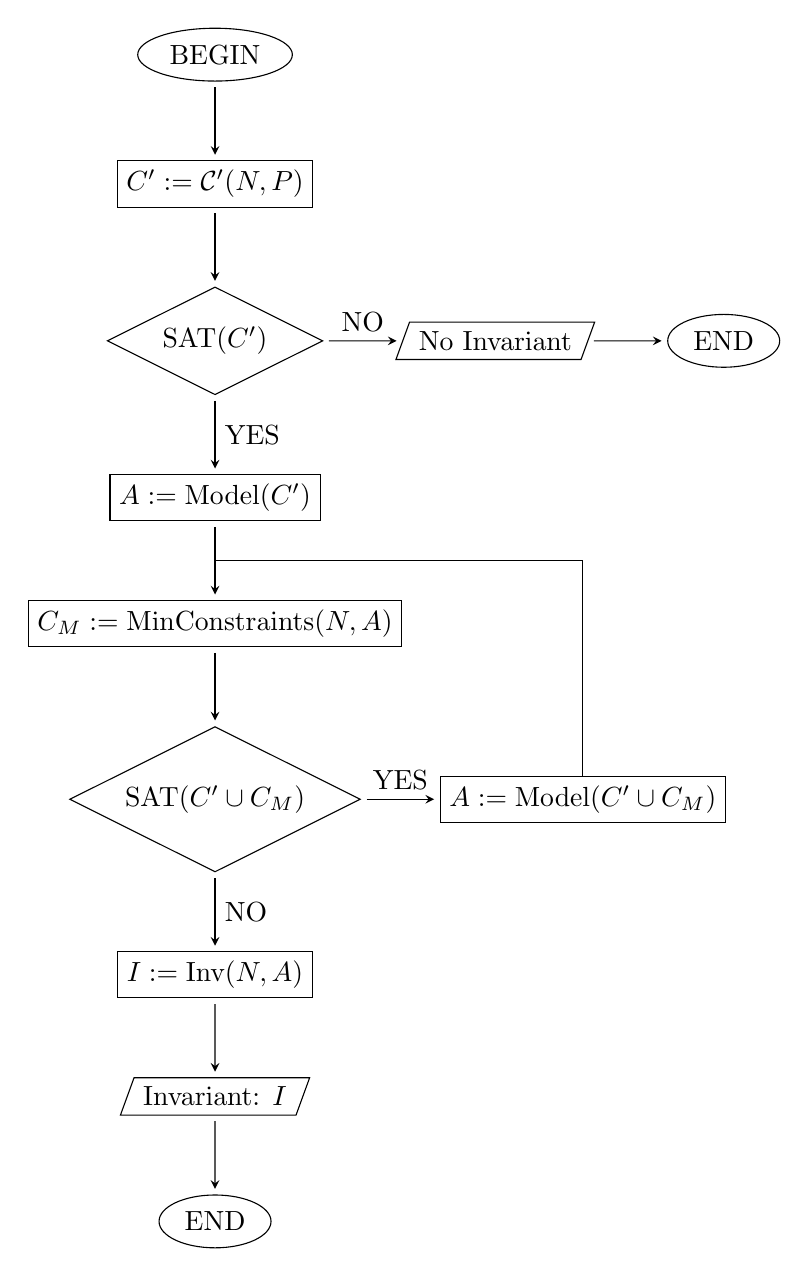
\begin{tikzpicture}
    \node[state] (begin) {BEGIN};
    \node[action, below=of begin] (c) {$C':=\mathcal C'(N, P)$};
    \node[decision, below=of c] (satc) {$\text{SAT}(C')$};
    \node[print, right=of satc] (noinv) {No Invariant};
    \node[action, below=of satc] (model1) {$A:=\text{Model}(C')$};
    \node[action, below=of model1] (cm) {$C_M:=\text{MinConstraints}(N, A)$};
    \node[decision, below=of cm] (satcm) {$\text{SAT}(C' \cup C_M)$};
    \node[action, right=of satcm] (model2) {$A:=\text{Model}(C' \cup C_M)$};
    \node[action, below=of satcm] (inv) {$I := \text{Inv}(N, A)$};
    \node[print, below=of inv] (printinv) {Invariant: $I$};
    \node[state, right=of noinv] (end1) {END};
    \node[state, below=of printinv] (end2) {END};
    
    \draw (begin) edge (c);
    \draw (c) edge (satc);
    \draw (satc) edge node[above]{NO} (noinv);
    \draw (noinv) edge (end1);
    \draw (satc) edge node[right]{YES} (model1);
    \draw (model1) edge coordinate[pos=.5] (edgein) (cm);
    \draw (cm) edge (satcm);
    \draw (satcm) edge node[above]{YES} (model2);
    \draw (model2) |- (edgein);
    \draw (satcm) edge node[right]{NO} (inv);
    \draw (inv) edge (printinv);
    \draw (printinv) edge (end2);
  \end{tikzpicture}
\end{center}

\begin{verbatim}
* Property of minimization constraints C_M generated from A: 
    If A' satisfies C' u C_M, then Inv(N, A') uses less places than Inv(N, A)
\end{verbatim}

\newpage
\begin{verbatim}
* Example:
  - Dual state constraints C' and satisfying assignment A for C' as in example for method Invariant

  - Minimization constraints:

    nc  ~= 0 => m_nc = 1
    |           --------
    |              |
    |           place appears in invariant
    |
    place coefficient in the invariant

    nc   = 0 => m_nc  = 0
    |           ---------
    |              |
    |           place does not appear in invariant
    |
    place coefficient in the invariant

    m   ~= 0 => m_m   = 1
    m    = 0 => m_m   = 0
    cs1 ~= 0 => m_cs1 = 1
    cs1  = 0 => m_cs1 = 0
    cs2 ~= 0 => m_cs2 = 1
    cs2  = 0 => m_cs2 = 0

    m_nc + m_m + m_cs1 + m_cs2 < 3
    --------------------------   |
                |                |
                |    number of places appearing in current invariant for A
                |    = #{s | A(s) ~= 0} = #{m, cs1, cs2}
                |
                |
  number of places appearing in new invariant
\end{verbatim}

\begin{verbatim}
* Subprocedure \text{MinConstraints}:

  Input:
    (S, T, E, M0) : Petri net
    A             : Assignment
  Output:
    C_M           : Minimization Constraints

Input:
 N   = (S, T, E, M0)
     = ( (nc m cs1 cs2) (t1 t2 t3 t4) (e1 ... en) (2 1 0 0) )
 A   = ( nc=0, m=1, cs1=1, cs2=1, target1=1 )

TODO: Unroll pseudocode?

\end{verbatim}

\newpage

\section{Method Safety by Refinement}

The method Safety by Refinement applies trap conditions to check that a given Petri net \verb=N= never violates a property \verb=P=.
We present the method Invariant by example on a mutual exclusion algorithm by Delzanno2001.

\begin{verbatim}

* Code

bool m1 = false;
bool m2 = false;

// Thread 1:
while (true) {
  if (! m2 && ! test_and_set(m1)) {
    // critical section 1
    m1 = false
  }
  if (! m1 && ! test_and_set(m2)) {
    // critical section 2
    m2 = false
  }
}

// Thread 2:
while (true) {
  if (! m2 && ! test_and_set(m1)) {
    // critical section 1
    m1 = false
  }
  if (! m1 && ! test_and_set(m2)) {
    // critical section 2
    m2 = false
  }
}

Property: Thread 1 and Thread 2 are never in any critical section at the same time.

* Petri net:
\end{verbatim}
\begin{center}
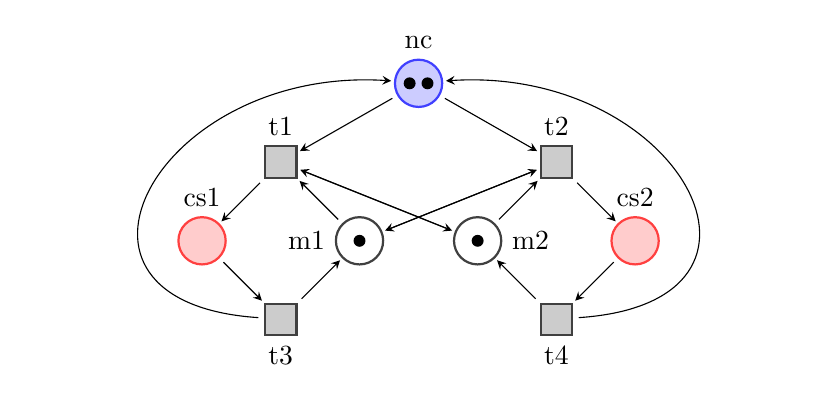
\begin{tikzpicture}[node distance=2cm]
  \node[blue place, tokens=2, label=above:nc] (nc) {};
  \node[place, tokens=1, label=right:m2, below of=nc, xshift=+0.75cm] (s2) {};
  \node[place, tokens=1, label=left:m1, below of=nc, xshift=-0.75cm] (s1) {};
  \node[red place, label=above:cs1, left of=s1] (cs1) {};
  \node[red place, label=above:cs2, right of=s2] (cs2) {};
  \node[transition, label=above:t1] (t1) at ($(s1)!0.5!(cs1) + (0,1cm)$) {}
	edge [pre] (nc)
	edge [pre] (s1)
	edge [pre] (s2)
	edge [post] (cs1)
	edge [post] (s2);
  \node[transition, label=above:t2] (t2) at ($(s2)!0.5!(cs2) + (0,1cm)$) {}
	edge [pre] (nc)
	edge [pre] (s2)
	edge [pre] (s1)
	edge [post] (cs2)
	edge [post] (s1);
  \node[transition, label=below:t3] (t3) at ($(s1)!0.5!(cs1) - (0,1cm)$) {}
	edge [pre] (cs1)
	edge [post] (s1)
	edge [post,bend left,min distance=3cm, out=115, in=115] (nc);
  \node[transition, label=below:t4] (t4) at ($(s2)!0.5!(cs2) - (0,1cm)$) {}
	edge [pre] (cs2)
	edge [post] (s2)
	edge [post,bend right,min distance=3cm, out=-115, in=-115] (nc);
\end{tikzpicture}
\end{center}

\newpage
\begin{verbatim}
* Method Safety by Refinement:

  Subprocedure TrapConditions constructs trap conditions C_\theta corresponding to N and A.
  Subprocedure \Delta constructs refinement constraint \delta corresponding to A_\theta.
\end{verbatim}
\begin{center}
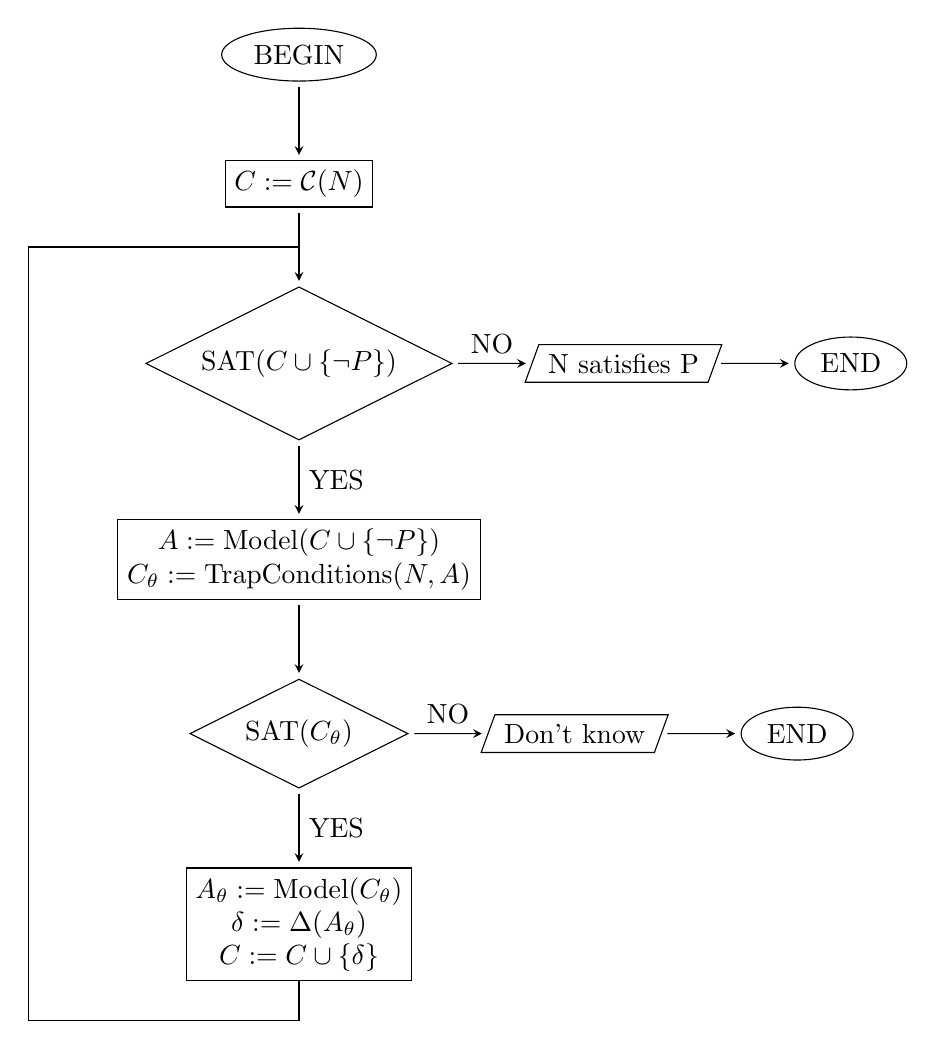
\begin{tikzpicture}
  \node[state] (begin) {BEGIN};
  \node[action, below=of begin] (c) {$C:=\mathcal C(N)$};
  \node[decision, below=of c] (satc) {$\text{SAT}(C \cup \{\neg P\})$};
  \node[action, below=of satc] (modelc) {$A:=\text{Model}(C \cup \{\neg P\})$\\
                               	$C_{\theta}:=\text{TrapConditions}(N, A)$};
  \node[decision, below=of modelc] (satctheta) {$\text{SAT}(C_\theta)$};
  \node[action, below=of satctheta] (modelctheta) {$A_\theta:=\text{Model}(C_\theta)$\\
                                    	$\delta:=\Delta(A_\theta)$\\
                                    	$C:=C \cup \{\delta\}$};
  \node[print, right=of satc] (yes) {N satisfies P};
  \node[print, right=of satctheta] (dontknow) {Don't know};
  \node[state, right=of yes] (end1) {END};
  \node[state, right=of dontknow] (end2) {END};

  \draw (begin) edge (c);
  \draw (c) edge coordinate[pos=.5] (edgein) (satc);
  \draw (satc) edge node[above]{NO} (yes);
  \draw (yes) edge (end1);
  \draw (satc) edge node[right]{YES} (modelc);
  \draw (modelc) edge (satctheta);
  \draw (satctheta) edge node[above]{NO} (dontknow);
  \draw (dontknow) edge (end2);
  \draw (satctheta) edge node[right]{YES} (modelctheta);
  \draw (modelctheta.south) -- ([yshift=-0.5cm] modelctheta.south)
  -| ([xshift=-2cm] modelctheta.west) |- (edgein);
\end{tikzpicture}
\end{center}

\begin{verbatim}
* Property of trap conditions C_\theta: If C_\theta is sat then there is a set S such that
  1. S is a trap in the net N
  2. S is marked in the initial marking M0
  3. S is unmarked in the assignment A

* Property of A_\theta: for each place s, A_\theta(s) iff s \in S

* Property of refinement constraint \delta: Constraint \delta refines the abstraction, i.e.
  1. A ^ \delta is unsat (\delta excludes A)
  2. N |= \delta is sat  (\delta is a property of N)
\end{verbatim}

\newpage
\begin{verbatim}
* Example
  - State constraints C:
    nc  =  2 - t1 - t2 + t3 + t4
    m1  =  1 - t1 + t3
    m2  =  1 - t2 + t4
    cs1 =  0 + t1 - t3
    cs2 =  0 + t2 - t4
    nc  >= 0
    m1  >= 0
    m2  >= 0
    cs1 >= 0
    cs2 >= 0
    t1  >= 0
    t2  >= 0
    t3  >= 0
    t4  >= 0

  - Assignment A:
    nc  = 0
    m1  = 0
    m2  = 0
    cs1 = 1
    cs2 = 1
    t1  = 1
    t2  = 1
    t3  = 0
    t4  = 0

  - Trap conditions C_\theta:

    - Trap implications:

    cs1 => m1 \/ nc
    ^      ^     ^
    |      |     |
    |      |     nc \in S
    |      |
    |      m1 \in S
    |
    cs1 \in S
    
    cs2 => m2 \/ nc
    nc  => (m2 \/ cs1) /\ (m1 \/ cs2)
    m1  => (m2 \/ cs1) /\ (m1 \/ cs2)
    m2  => (m2 \/ cs1) /\ (m1 \/ cs2)

    - At least one of the intially marked places belongs to S:
    nc \/ m1 \/ m2

    - None of the marked places in A belongs to S:
    ~cs1 /\ ~cs2

  - Assignment A_\theta:
    nc  = false
    m1  = true
    m2  = true
    cs1 = false
    cs2 = false
\end{verbatim}

\newpage
\begin{verbatim}
  - Refinement constraint \delta:
    m1 + m2 >= 1
    ^    ^
    |    |
    ------
      |
      S = {m1, m2}, therefore \delta excludes assignment A in the next iteration

* Trap implication:

  place s \in S =>    /\       \    /
                     /  \       \  /     place p \in S
                    /    \       \/
                   t \in s*   p \in t*   


  "if s is in trap S then for each output transition t at least one successor p is in trap S"


* Refinement constraint \delta:

  \Sigma s >= 1  
  A(s)

  "At least one place in S is always marked"


* Subprocedure TrapConditions:

  Input:
    (S, T, E, M0) : Petri net
    A             : Satisfying assignment for C \cup { ~P }
  Output:
    C_\theta      : Trap conditions

  TODO: Unroll pseudocode?

* Subprocedure \Delta:

  Input:
    A_\theta      : Satisfying assignment for C_\theta
  Output:
    \delta        : Refinement constraint \delta

  TODO: Unroll pseudocode?
\end{verbatim}

\newpage
\section{Benchmarks of \bfc}

We experimented on the benchmarks \ttt{cprover-PN} and
\ttt{cprover\_software\_analysis} available at \\
\ttt{http://www.mpi-sws.org/\~{}jkloos/iic-experiments/cprover.zip}.
The set of benchmarks consists 77 benchmarks, 26 positive and 51 negative.
Table~\ref{bfc-experiments} shows the corresponding experimental results.

\begin{table}[h]
\begin{center}
  \begin{tabular}{ | p{7cm} | r | r | r | r | } %
    \hline
    Method & pos & neg & don't know & TO \\
    \hline
    Safety (over real numbers or naturals)      & 23 &  0 & 54 &  0 \\
    Invariant \& Invariant with Minimization    & 23 &  0 & 54 &  0 \\
    Safety by Refinement                        & 23 &  0 & 54 &  0 \\
    \hline
  \end{tabular}
\end{center}
\caption{Experimental results for the benchmarks of \bfc}
\label{bfc-experiments}
\end{table}

\section{Benchmarks of \mist}

We experimented on the benchmarks available at \\
\ttt{https://github.com/pierreganty/mist/tree/master/examples/boundedPN}
and \\
\ttt{https://github.com/pierreganty/mist/tree/master/examples/PN}.
The set of benchmarks consists 27 benchmarks, 23 positive and 4 negative.
Table~\ref{mist-experiments} shows the corresponding experimental results.

\begin{table}[h]
\begin{center}
  \begin{tabular}{ | p{6cm} | r | r | r | r | }
    \hline
    Method & pos & neg & don't know & TO \\
    \hline
    Safety (over real numbers or naturals)      & 14 &  0 & 13 &  0 \\
    Invariant \& Invariant with Minimization    & 14 &  0 & 13 &  0 \\
    Safety by Refinement                        & 20 &  0 &  7 &  0 \\
    \hline
  \end{tabular}
\end{center}
\caption{Experimental results for the benchmarks of \mist}
\label{mist-experiments}
\end{table}

\section{Benchmarks of \iic}

We experimented on the benchmarks available at \\
\ttt{https://svn.rse.mpi-sws.org/RSE/IC3forWSTS/code/trunk/examples/soter}.
The set of benchmarks consists 38 benchmarks, 28 positive and 10 negative.
Table~\ref{iic-experiments} shows the corresponding experimental results.

\begin{table}[h]
\begin{center}
  \begin{tabular}{ | p{6cm} | r | r | r | r | }
    \hline
    Method & pos & neg & don't know & TO \\
    \hline
    Safety (over real numbers or naturals)      & 2 & 0 & 36 & 0 \\
    Invariant \& Invariant with Minimization    & 2 & 0 & 26 & 0 \\
    Safety by Refinement                        & 2 & 0 & 36 & 0 \\
    \hline
  \end{tabular}
\end{center}
\caption{Experimental results for the benchmarks of \iic}
\label{iic-experiments}
\end{table}

We constructed the following two invariants by applying the method
Invariant with Minimization.

\begin{itemize}
\item \verb?firewall__no_pred_called_with_zero__depth_1__fixed?: \verb?(assert (<= l739 0))?
\item \verb?firewall__no_pred_called_with_zero__depth_2__fixed?: \verb?(assert (<= l3849 0))?
\end{itemize}

\iic\ constructs the following two invariants.

\begin{itemize}
\item \verb=firewall__no_pred_called_with_zero__depth_1__fixed.spec=: \verb=(l739 < 1)=
\item \verb=firewall__no_pred_called_with_zero__depth_2__fixed.spec=: \verb=(l3849 < 1)=
\end{itemize}

\fi

\end{document}
